\documentclass[review]{elsarticle} %review=doublespace preprint=single 5p=2 column
%%% Begin My package additions %%%%%%%%%%%%%%%%%%%
\usepackage[hyphens]{url}
\usepackage{lineno} % add 
\linenumbers % turns line numbering on 
\bibliographystyle{elsarticle-harv}
\biboptions{sort&compress} % For natbib
\usepackage{graphicx}
\usepackage{booktabs} % book-quality tables
%% Redefines the elsarticle footer
\makeatletter
\def\ps@pprintTitle{%
 \let\@oddhead\@empty
 \let\@evenhead\@empty
 \def\@oddfoot{\it \hfill\today}%
 \let\@evenfoot\@oddfoot}
\makeatother

% A modified page layout
\textwidth 6.75in
\oddsidemargin -0.15in
\evensidemargin -0.15in
\textheight 9in
\topmargin -0.5in
%%%%%%%%%%%%%%%% end my additions to header



\usepackage[T1]{fontenc}
\usepackage{lmodern}
\usepackage{amssymb,amsmath}
\usepackage{ifxetex,ifluatex}
\usepackage{fixltx2e} % provides \textsubscript
% use upquote if available, for straight quotes in verbatim environments
\IfFileExists{upquote.sty}{\usepackage{upquote}}{}
\ifnum 0\ifxetex 1\fi\ifluatex 1\fi=0 % if pdftex
  \usepackage[utf8]{inputenc}
\else % if luatex or xelatex
  \usepackage{fontspec}
  \ifxetex
    \usepackage{xltxtra,xunicode}
  \fi
  \defaultfontfeatures{Mapping=tex-text,Scale=MatchLowercase}
  \newcommand{\euro}{€}
\fi
% use microtype if available
\IfFileExists{microtype.sty}{\usepackage{microtype}}{}
\usepackage{graphicx}
% We will generate all images so they have a width \maxwidth. This means
% that they will get their normal width if they fit onto the page, but
% are scaled down if they would overflow the margins.
\makeatletter
\def\maxwidth{\ifdim\Gin@nat@width>\linewidth\linewidth
\else\Gin@nat@width\fi}
\makeatother
\let\Oldincludegraphics\includegraphics
\renewcommand{\includegraphics}[1]{\Oldincludegraphics[width=\maxwidth]{#1}}
\ifxetex
  \usepackage[setpagesize=false, % page size defined by xetex
              unicode=false, % unicode breaks when used with xetex
              xetex]{hyperref}
\else
  \usepackage[unicode=true]{hyperref}
\fi
\hypersetup{breaklinks=true,
            bookmarks=true,
            pdfauthor={},
            pdftitle={No indicators for stochastic transitions but establishing baselines for early warning signals remains a general challenge},
            colorlinks=true,
            urlcolor=blue,
            linkcolor=magenta,
            pdfborder={0 0 0}}
\urlstyle{same}  % don't use monospace font for urls
\setlength{\parindent}{0pt}
\setlength{\parskip}{6pt plus 2pt minus 1pt}
\setlength{\emergencystretch}{3em}  % prevent overfull lines
\setcounter{secnumdepth}{0}
% Pandoc toggle for numbering sections (defaults to be off)
\setcounter{secnumdepth}{0}
% Pandoc header



\begin{document}
\begin{frontmatter}
  \title{No indicators for stochastic transitions but establishing baselines for
         early warning signals remains a general challenge}
  \author[cstar]{Carl Boettiger\corref{cor1}}
  \cortext[cor1]{Corresponding author}
  \ead{cboettig@ucsc.edu}
  \address[cstar]{Center for Stock Assessment Research, Department of Applied Math and Statistics, University of California, Mail Stop SOE-2, Santa Cruz, CA 95064, USA}
  \author[esp]{Alan Hastings}
  \address[esp]{Department of Environmental Science and Policy, University of California, Davis, CA, 95616 United States}
 \end{frontmatter}


In Boettiger \& Hastings {[}1{]} we demonstrated that conditioning on
observing a purely stochastic transition from one stable basin to
another could generate time-series trajectories that could be mistaken
for an early warning signal of a critical transition (such as might be
due to a fold bifurcation; {[}2{]}, when instead the shift is merely due
to chance. While the goal was to highlight a potential danger in mining
historical records for patterns showing sudden shifts when seeking to
test early warning techniques, Drake {[}3{]} draws attention to a
potentially more interesting consequence of our analysis. Drake argues
that the bias observed could be used to forecast purely stochastic
transitions -- a task previously thought to be impossible (e.g.
@Ditsleven2010, also Reference 4 for a brief overview of other
examples). Unfortunately, we feel this interpretation too generous and
must agree with the prevailing opinion that early warning signals for
purely stochastic transitions do not exist. Drake demonstrates how the
patterns presented in {[}1{]} show an indisputable difference between
the time series that transition by chance and the much larger population
of replicate time series driven by the identical mechanism that do not
transition by chance. We show that this pattern in question is a
consequence of any large deviation, and not caused by or indicative of
any impending shift to an alternative stable state.

We here provide a numerical demonstration that the pattern in question
for consideration of an early warning signal appears not only before
purely stochastic transitions (as seen in Reference 1) but also in large
deviations from a single stable point, in which no such transition is
possible.

We replicate the analysis of Boettiger and Hastings {[}1{]} using time
series replicates produced by an Ornstein-Uhlenbeck (OU) process: a
stochastic differential equation in which there is only a single optimum
whose strength is proportional to the displacement,

\[ dX = - \alpha X dt + \sigma dBt \]

Instead of conditioning on trajectories that experience a large
deviation, we condition on trajectories that experience a very large
deviation. We then compute warning signals for each of these large
deviation trajectories, and compare their distribution to that of the
entire population of trajectories as shown in Figure 1. We note that the
same bias is observed. This should help illustrate that observations we
reported are driven by the large deviation preceding the transition, and
are simply evidence of this fact and not of an impending transition per
se. While trajectories already far from the origin are more likely to
transition than ones close to the average, such events can be trivially
identified by comparing their states to the historical average.

\begin{figure}[htbp]
\centering
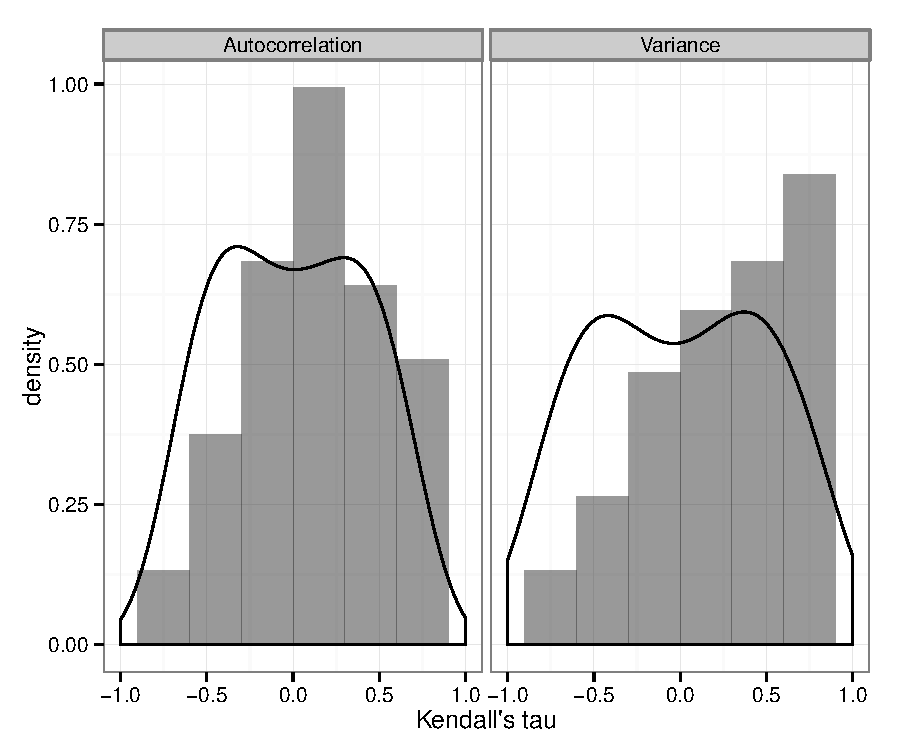
\includegraphics{figure1.pdf}
\caption{Figure 1. Histogram shows the frequency the correlation
statistic $\tau$ observed for each warning signal (variance,
autocorrelation coefficient) on the large deviation samples. Background
distribution of all samples show by smooth line (kernel density
estimate). More positive values of tau are supposed to indicate a rising
indicator which can be a signal of an approaching transition {[}2{]}.
$\alpha = 5$, $\sigma=3.5$, $t \in (0, 10)$, 2000 replicates, 20,000
sample points each. Conditionally selected trajectories experiencing a
deviation of at least -4, and analyzed the 1,500 data points prior to
the threshold to determine a warning signal (following Reference 5).
(\href{https://raw.github.com/cboettig/earlywarning/7460ea94c293844d8e88c83b95e3d80004817de6/inst/examples/beer.md}{link
to code},
\href{https://raw.github.com/cboettig/earlywarning/7460ea94c293844d8e88c83b95e3d80004817de6/inst/examples/beer_nulldat.csv}{null
distribution data},
\href{https://raw.github.com/cboettig/earlywarning/7460ea94c293844d8e88c83b95e3d80004817de6/inst/examples/beer_dat.csv}{conditional
distribution data})}
\end{figure}

Observing the bias shown in Figure 1 depends on having a rapid enough
sample frequency to capture the escape trajectory and a long enough
trajectory for the statistic to demonstrate an increase over time. Since
large deviations due to stochastic forces alone must be fast so must the
accompanying warning signal and managemnt response, which will show up
on the time scale of the perturbation. Of course fast relative to the
system dynamics, may or may not be fast relative to the timescale of
management; just as in the case of bifurcation-driven warning signals
(see Reference 6).

One might consider this a corallary of the Prosecutor's Fallacy we
originally presented, which demonstrated that examples of sudden
transitions historically selected from the literature could be mistaken
for positive evidence of early warning signals when they were in fact
due to purely stochastic transitions. Here we have seen how any large
deviation could be similarly misleading, whether or not it results in a
stochastic transition to an alternative stable state. From a classical
result of the large deviation theory one can gain considerable intuition
about why these chance deviations show much higher variance and
autocorrelation than expected from the stationary distribution of a
stable point. Though large deviations are rare -- the time we must wait
to observe a deviation of size $L$ in the system above scales as
$\exp\left(L^2/\sigma^2\right)$ (the familiar Ahrennius relationship),
when these deviations occur they occur very rapidly. The expected time
for an exersion to a distant point $L$ that does not again cross the
stable point before reaching $L$ scales as $\log(L/\sigma)$, just as a
trajectory returing down the gradient of the attractor from $L$ to the
stable point (proofs in Reference 7 or Reference 8). While most
trajectories in the stationary distribution take steps in each direction
with equal probability, these large deviations moving rapidly to the
boundary will consequently show the much greater autocorrelation, and in
achieving a much greater deviation than typically observed, also show
the spike in variance we observe. That such trajectories appear to be
pulled in the direction of their escape rather than climbing away
against a restorative force has led to confusion before. Reference 8
argues how this shows how a ``punctuated equilibrium'' pattern of statis
followed by rapid change could arise entirely from small steps, and
Reference 9 empirically demonstrates this phenomena in the trajectories
of local population extinctions.

In conclusion, we heartily agree with the need for a decision-theoretic
approach to early warning signal questions {[}10{]}. Central to a
decision-theoretic approach is enumerating alternative scenarios that
are possible given the observed data. We have highlighted how purley
stochastic transitions and large deviations are such possiblities. The
challenge of sufficient or unique early warning indicators is not
limited to stochastic shifts, but includes the more typical critical
transitions. For instance, rising variance or autocorrelation patterns
typical of fold bifurcations can be observed in more benign bifurcations
or smooth transitions {[}11{]}. Early warning signals may offer a
promising technique that will one day allow us to avoid seemingly
unpredictable catastrophes -- but we must not lose sight of just how
difficult are the challenges involved. A key step here and for early
warning indicators more generally is to understand these other
circumstances in which they can arise, that we may then develop ways to
eliminate those possibilities. Though we may never be able to detect
purely stochastic transitions, perhaps these approaches in this
discussion may lead to more unique and sufficient indicators for true
critical transitions.

1 Boettiger, C. \& Hastings, A. 2012 Early warning signals and the
prosecutor's fallacy. \emph{Proceedings of the Royal Society B:
Biological Sciences} (doi:10.1098/rspb.2012.2085)

2 Scheffer, M. et al. 2009 Early-warning signals for critical
transitions. \emph{Nature} \textbf{461}, 53--9.

3 Drake, J. M. 2013 Early warning signals of stochastic switching.
\emph{Proceedings of The Royal Society B} \textbf{in press}.

4 Lenton, T. M. 2011 Early warning of climate tipping points.
\emph{Nature Climate Change} \textbf{1}, 201--209.
(doi:10.1038/nclimate1143)

5 Dakos, V., Scheffer, M., van Nes, E. H., Brovkin, V., Petoukhov, V. \&
Held, H. 2008 Slowing down as an early warning signal for abrupt climate
change. \emph{Proceedings of the National Academy of Sciences}
\textbf{105}, 14308--12. (doi:10.1073/pnas.0802430105)

6 Hughes, T. P., Linares, C., Dakos, V., van de Leemput, I. a \& van
Nes, E. H. 2013 Living dangerously on borrowed time during slow,
unrecognized regime shifts. \emph{Trends in ecology \& evolution}
\textbf{28}, 149--55. (doi:10.1016/j.tree.2012.08.022)

7 Ludwig, D. 1981 Escape from Domains of Attraction for Sytstems
Perturbed by Noise. In \emph{Nonlinear Phenomena in Physics and Biology}
(eds R. H. Enns B. L. Jones R. M. Miura \& S. S. Rangnekar), pp.
549--566. Boston, MA: Springer New York.

8 Lande, R. 1985 Expected time for random genetic drift of a population
between stable phenotypic states. \emph{Proceedings of the National
Academy of Sciences} \textbf{82}, 7641--7645.

9 Drake, J. M. \& Griffen, B. D. 2009 Speed of expansion and extinction
in experimental populations. \emph{Ecology letters} \textbf{12}, 772--8.
(doi:10.1111/j.1461-0248.2009.01325.x)

10 Boettiger, C. \& Hastings, A. 2012 Quantifying limits to detection of
early warning for critical transitions. \emph{Journal of The Royal
Society Interface} \textbf{9}, 2527--2539. (doi:10.1098/rsif.2012.0125)

11 Kéfi, S., Dakos, V., Scheffer, M., Van Nes, E. H. \& Rietkerk, M.
2012 Early warning signals also precede non-catastrophic transitions.
\emph{Oikos} (doi:10.1111/j.1600-0706.2012.20838.x)

\end{document}


